%\newpage
\section{Laboratorio: Google Firebase} \label{lab4}

\paragraph{Obiettivo della lezione} Creazione di un evento RSVP per realizzare un invito interattivo, offrendo una chat per gli ospiti oltre ai dettagli dell'evento.\\
La caratteristica chiave dei PaaS è l'alto livello di astrazione garantito dalle estensioni (\textbf{add-ons}) che semplificano lo sviluppo dando l'opportunità di integrare funzionalità avanzate. 
Nella nostra applicazione integriamo l'auth tramite email:pass usando \textit{Firebase Authentication} e \textit{FirebaseUI}.
La chat è realizzata con \textit{Cloud Firestore} mentre la sicurezza per il database è garantita con \textit{Firebase Security rules}

\paragraph{\href{https://firebase.google.com/codelabs/firebase-get-to-know-web#0}{Tutorial creazione RSVP event}} durante tutto il procedimento abbiamo usato Stackblitz, un editor online in cui sono integrati workflows di Firebase. I file principali su cui lavoriamo sono \verb|index.js| e \verb|index.html|
\begin{enumerate}
    \item Come prima cosa creiamo un nuovo progetto Firebase:
    \begin{itemize}
        \item scegliere i metodi di autenticazione, noi abbiamo selezionato solo "Email/Password"
    \end{itemize}
    
    \item Creiamo un database, inizialmente in modalità "test", il che significa che il DB è aperto per letture e scritture. Più avanti nel codelab scriviamo le nostre regole di sicurezza custom made
    
    \item Al fine di utilizzare Firebase nell'app, importiamo varie librerie con degli \verb|import| statements in \verb|index.js|.\\
    E' fondamentale includere in \verb|index.js| anche il nostro oggetto di configurazione Firebase:
    \begin{lstlisting}[languague=Javascript]
    // Your web app's Firebase configuration
    const firebaseConfig = {
      apiKey: "your_api_key",
      authDomain: "labcloud-firebase.firebaseapp.com",
      projectId: "labcloud-firebase",
      storageBucket: "labcloud-firebase.appspot.com",
      messagingSenderId: "584194338624",
      appId: "1:584194338624:web:bc611483abd2b251c114a5",
      measurementId: "G-TY9GPL15Y6"
    };
    \end{lstlisting}

    \item Aggiungere accesso utente (\textbf{RSVP}): per aggiungere nuove features si deve
    \begin{enumerate}
        \item importare nuovi pacchetti dalle librerie
        \item modificare opportunamente \verb|index.html| (ad esempio aggiungere buttone per RSVP)
        \item aggiungere un \textbf{event listener} in \verb|index.js|
    \end{enumerate}
    
    \item Integrare la chat e archiviare tutti i messaggi inviati tramite \textbf{Cloud Firestore} (in pratica è un database NoSQL).  Ogni messaggio della chat viene archiviato come un documento dentro una raccolta chiamata \textit{guestbook} . Anche in questo caso occorre modificare l'html per includere un field nella pagina per scrivere i messaggi e un event listenere nel file js
    \begin{figure}[h!]
    \centering
    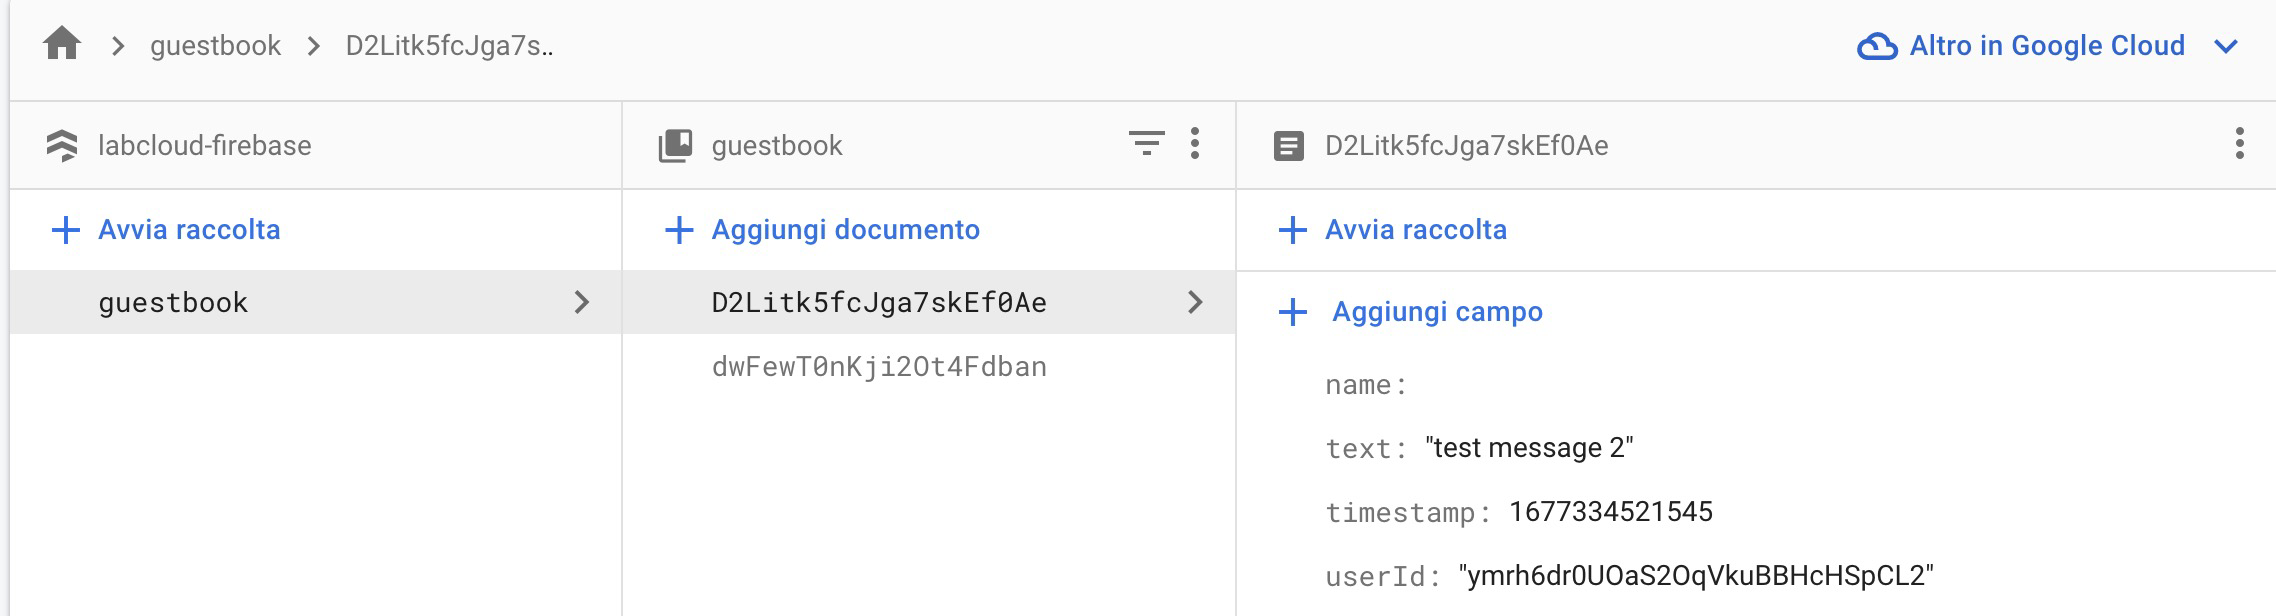
\includegraphics[width=0.7\textwidth]{18.png}
    \caption{Interfaccia che mostra i dettagli di ogni messaggio inviato nella chat}
    % \label{fig:enter-label}
\end{figure}

    \item Modifichiamo le \textbf{Rules} del DB:
    \begin{lstlisting}
    rules_version = '2';
    service cloud.firestore {
        match /databases/{database}/documents {
            match /guestbook/{entry} {
                allow read: if request.auth.uid != null;
                allow create:
                    if request.auth.uid == request.resource.data.userId;
            }
        }
    }
    \end{lstlisting}
    Per il libro degli ospiti solo gli utenti che hanno effettuato l'accesso possono leggere i messaggi (qualsiasi messaggio!), ma puoi creare un messaggio solo utilizzando il tuo ID utente.\\
    Inoltre, nel nostro esempio non consentiamo la modifica o l'eliminazione dei messaggi.

    \item Infine abbiamo aggiunto un bottone "\textit{Are you attending?}" per poter visualizzare quante persone hanno confermato la loro partecipazione
\end{enumerate}